    \chapter{Линейный рост {\it Macoma balthica}}
Рост особей рассматривается как отклик особей на совокупность условий обитания. 
Анализ роста проводили по усредненным возрастным рядам. 
Для их получения по каждому описанию   были   построены   треугольные   матрицы   (табл.~\ref{tab:Abram_sgl_growth_matrix}~--~\ref{tab:Porchnikha_sgl_growth_matrix},   Приложение~\ref{app:growth_matrix}),   полностью описывающие рост особей в поселении.

В   первую   очередь   анализ   был   проведен   по  усредненным   возрастным   рядам, построенным как взвешенная оценка (с учетом числа особей) характера роста всех генераций по   результатам   измерений   размеров  моллюсков  в   периоды   зимней   остановки   роста.  
Такая кумулятивная   характеристика   должна   в   наибольшей   мере   отражать   особенности   условий роста маком в каждом местообитании.
Наиболее длинный возрастной ряд удалось получить для среднего горизонта литорали губы Гаврилово --- $15$~лет при длине $17,9$~мм (табл.~\ref{tab:Gavrilovo_sgl_growth_matrix},   Приложение~\ref{app:growth_matrix}). 
Однако максимальный размер особей был отмечен в верхнем горизонте литорали губы Ярнышная --- $20,1$~мм при возрасте $13$~лет (табл.~\ref{tab:Yarnyshnaya_sgl_growth_matrix},   Приложение~\ref{app:growth_matrix}). 

Полученные   возрастные   ряды   были   аппроксимированы   с   помощью   уравнения Берталанфи   (рис.~\ref{ris:Barents_growth_gorizonts_all}).
    \begin{figure}[p]
        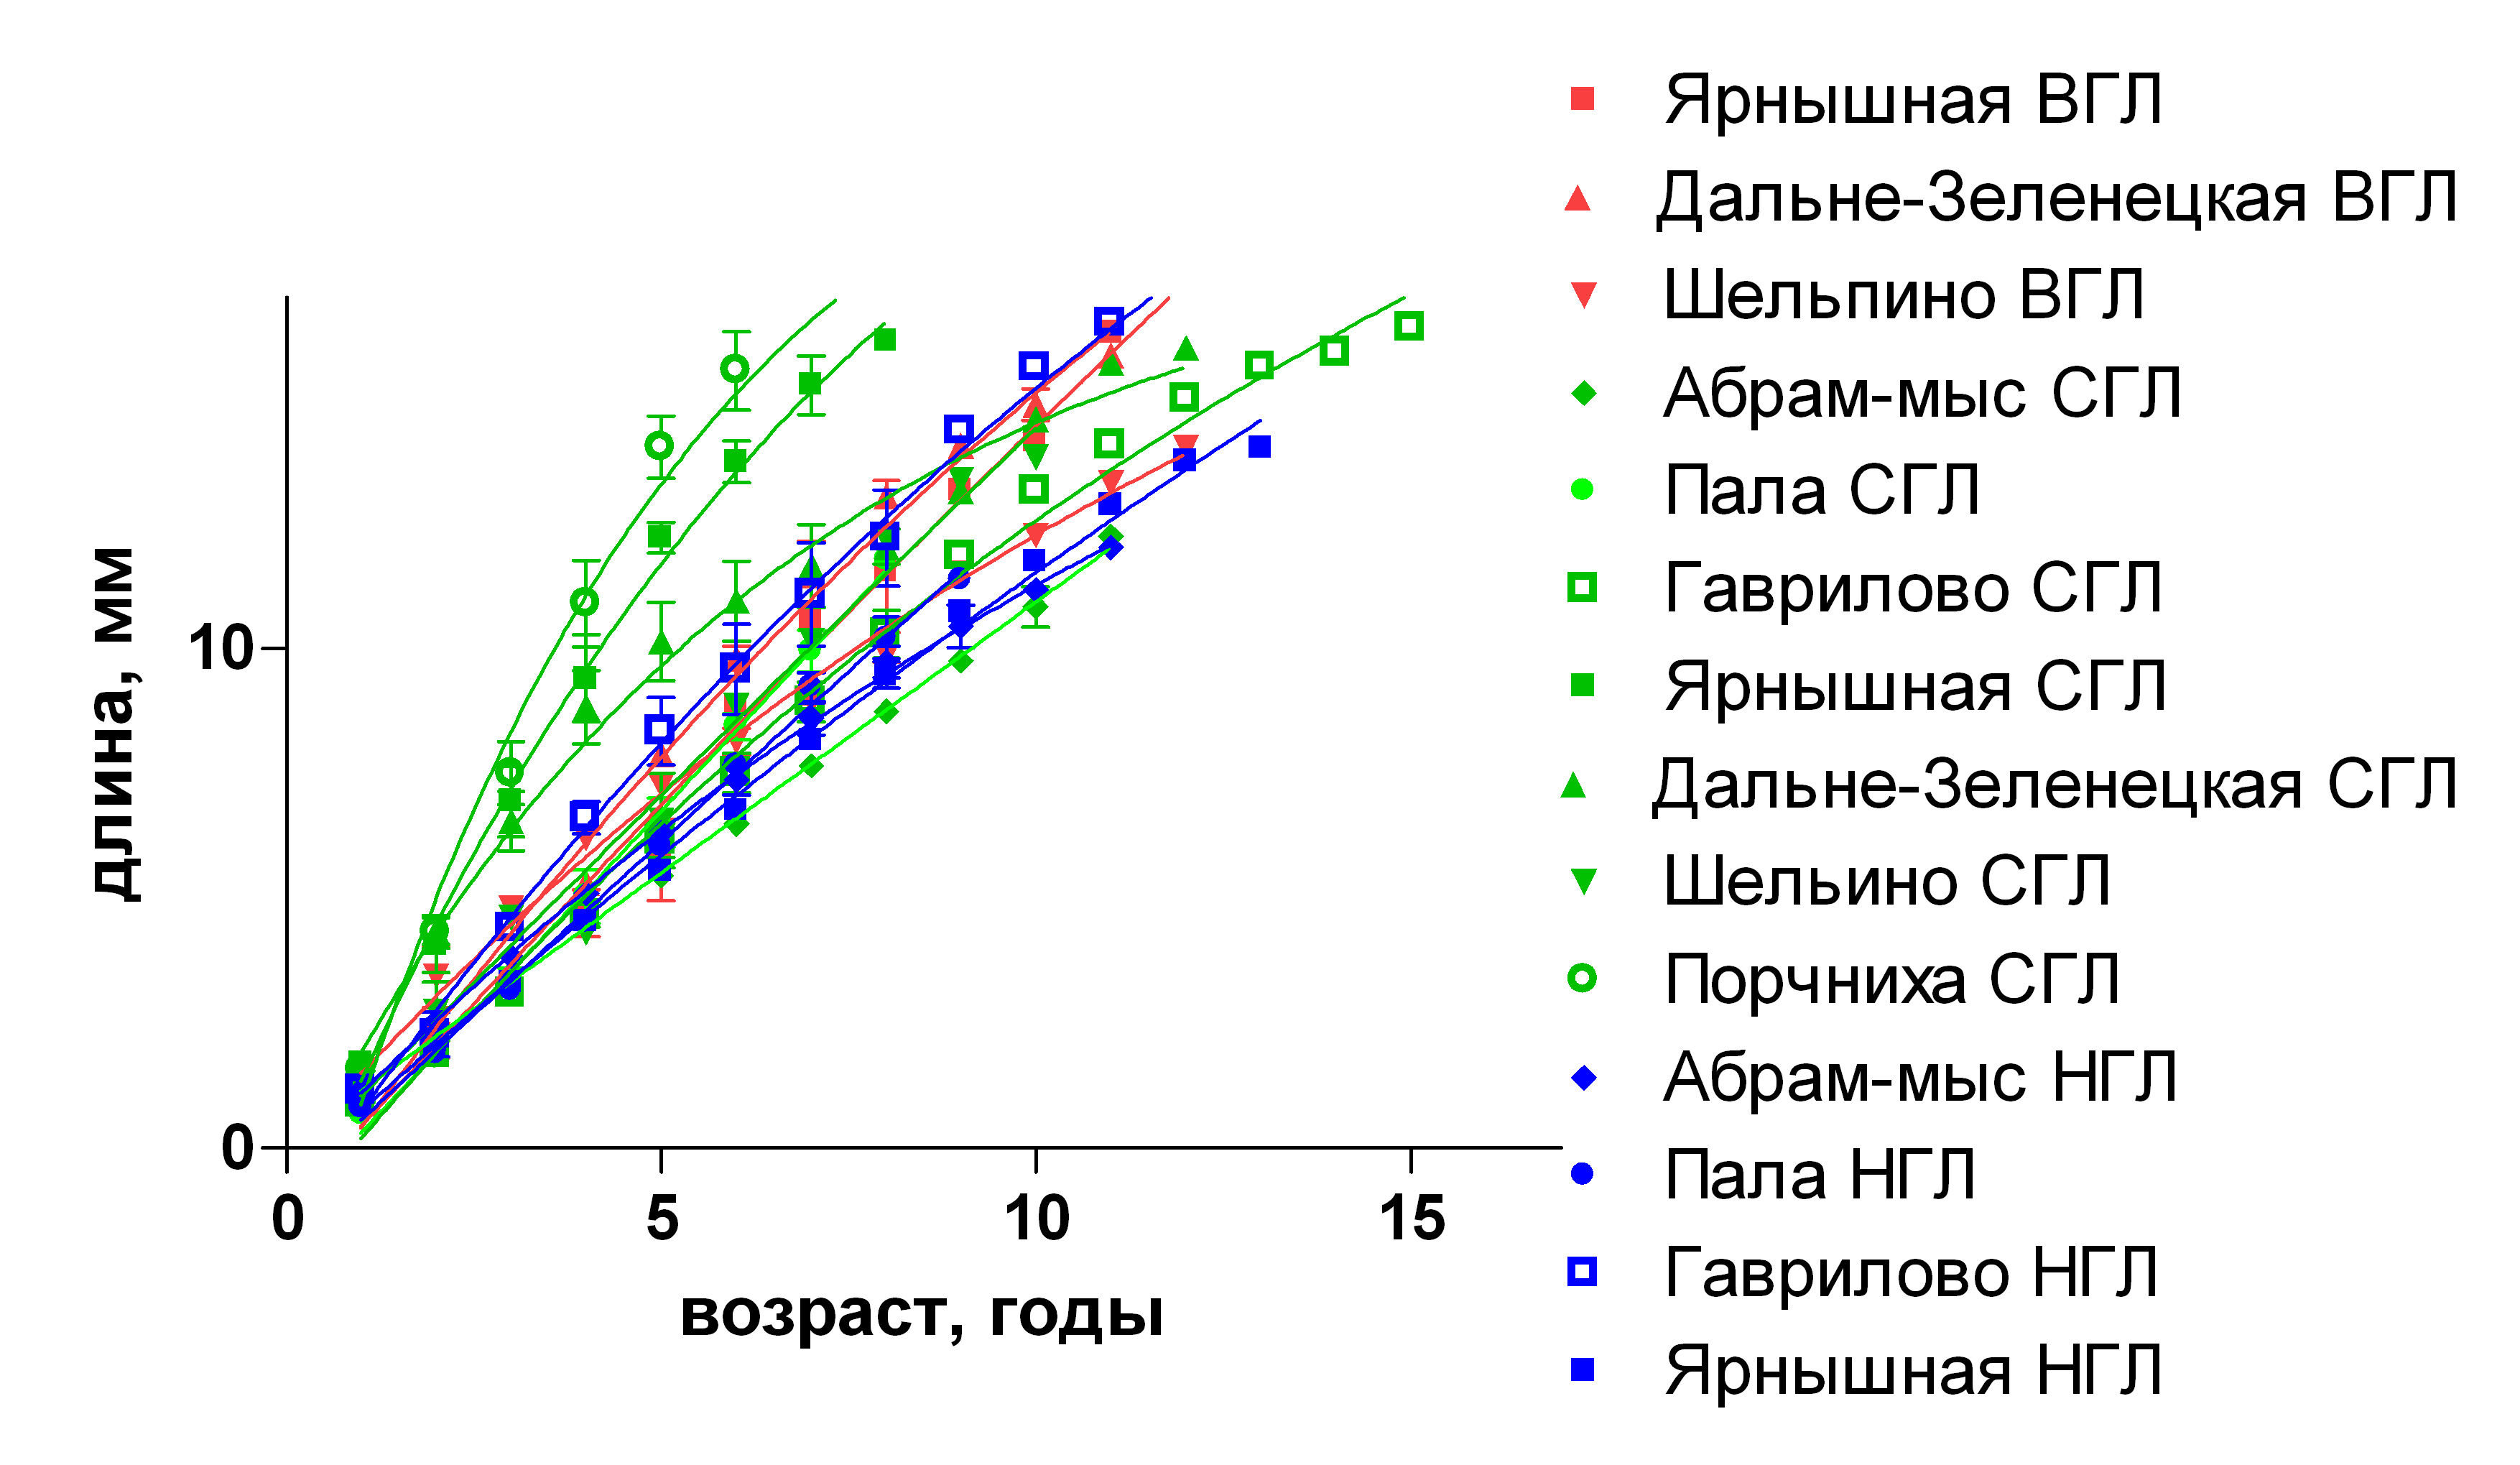
\includegraphics[width=\textwidth]{../Barenc_Sea/growth_from_MSc/Rost_gorizonts_all.jpg}
    \caption{Разнообразие моделей линейного роста, описывающих взвешенные характеристики возрастных рядов генераций в изученных поселениях маком}
    \label{ris:Barents_growth_gorizonts_all}
    \end{figure}

Быстрее   всего   росли   макомы   в   среднем   горизонте   литорали   губы Порчниха, достигая длины $19,4$~мм за $9$~лет и в среднем горизонте литорали губы Ярнышная --- $16,7$~мм за $8$~лет. 
Остальные кривые не распадаются на очевидные группы, и некоторые пересекают   друг   друга.   
Поэтому   была   использована   формальная   процедура   сравнения полученных   кривых   роста   с   учетом   разброса   эмпирических   данных   относительно регрессионной модели (рис.~\ref{ris:dendrogramma_linear_all_gorizonts}).
    \begin{figure}[p]
        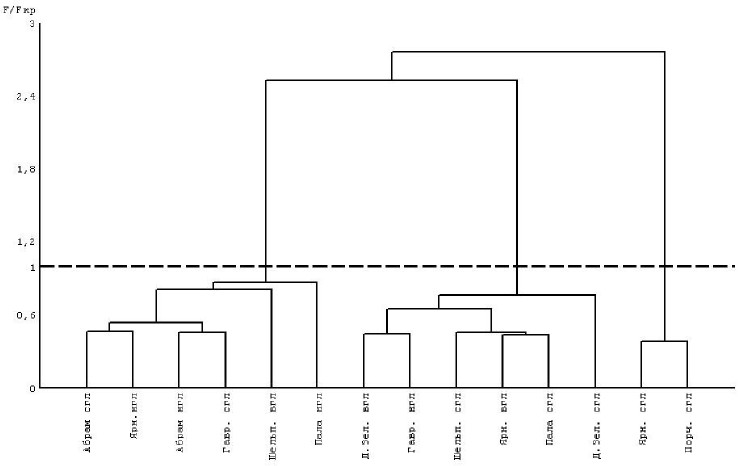
\includegraphics[width=\textwidth]{../Barenc_Sea/growth_from_MSc/dendrogramma_sravnenie_rosta_linear_all_gorizonts.jpg}
    \caption{Классификация поселений маком по моделям линейного роста, описывающих взвешенные характеристики возрастных рядов генераций}
    \label{ris:dendrogramma_linear_all_gorizonts}
    \end{figure}

В   ходе   классификации   было   выделено   три   кластера.   
В   первый   вошли   следующие описания (уровень различий внутри кластера менее $0,87$): Абрам-мыс, Пала-губа НГЛ, губа Гаврилово   СГЛ,   губа   Ярнышная   НГЛ,   Шельпино   ВГЛ.   
Второй   кластер   (уровень   различий внутри кластера менее $0,76$) составили участки Пала-губа СГЛ, губа Гаврилово НГЛ, губа Дальне-Зеленецкая,   губа   Ярнышная   ВГЛ,   Шельпино   СГЛ.   
В   последний   кластер   (уровень различий внутри кластера менее $0,38$) вошли участки губа Ярнышная СГЛ и губа Порчниха СГЛ. 

На участках Абрам-мыс и губа Дальне-Зеленецкая характер роста был одинаковый на всех горизонтах литорали. 
Однако в распределении остальных описаний нет географической приуроченности. 
Как и ожидалось, поселения  из средних горизонтов литорали губы Ярнышной и губы Порчниха   выделились   в   отдельный   кластер.   
Низкий   уровень   различий   ($0,38$)   говорит   о большом   разбросе   наблюдаемых   значений   относительно   модели   роста.   
Это   могло   бы свидетельствовать   об   относительно   грубом   описании   соответствующих   возрастных   рядов, хотя   значительный объем  выборки ($76$  и $65$  особей, соответственно)  позволяет  говорить  о значительном варьировании роста маком в пределах каждого участка.

Интересно,   что   при   незначительном   расхождении   кривых   роста,   уровень   различий между первым и вторым кластером оказался очень высоким ($2,52$). 
Не было отмечено явного разделения участков по мареографическому уровню, хотя во второй кластер попало больше описаний   с   более   высоких   горизонтов   литорали.   Максимальное   различие   было   между кластерами $2$ и $3$ ($2,76$).

По   итогам   классификации   было   выделено   три   группы   маком,   отличающиеся   по характеру роста (рис.~\ref{ris:Barents_clusters_gorizonts_all}).
    \begin{figure}[p]
        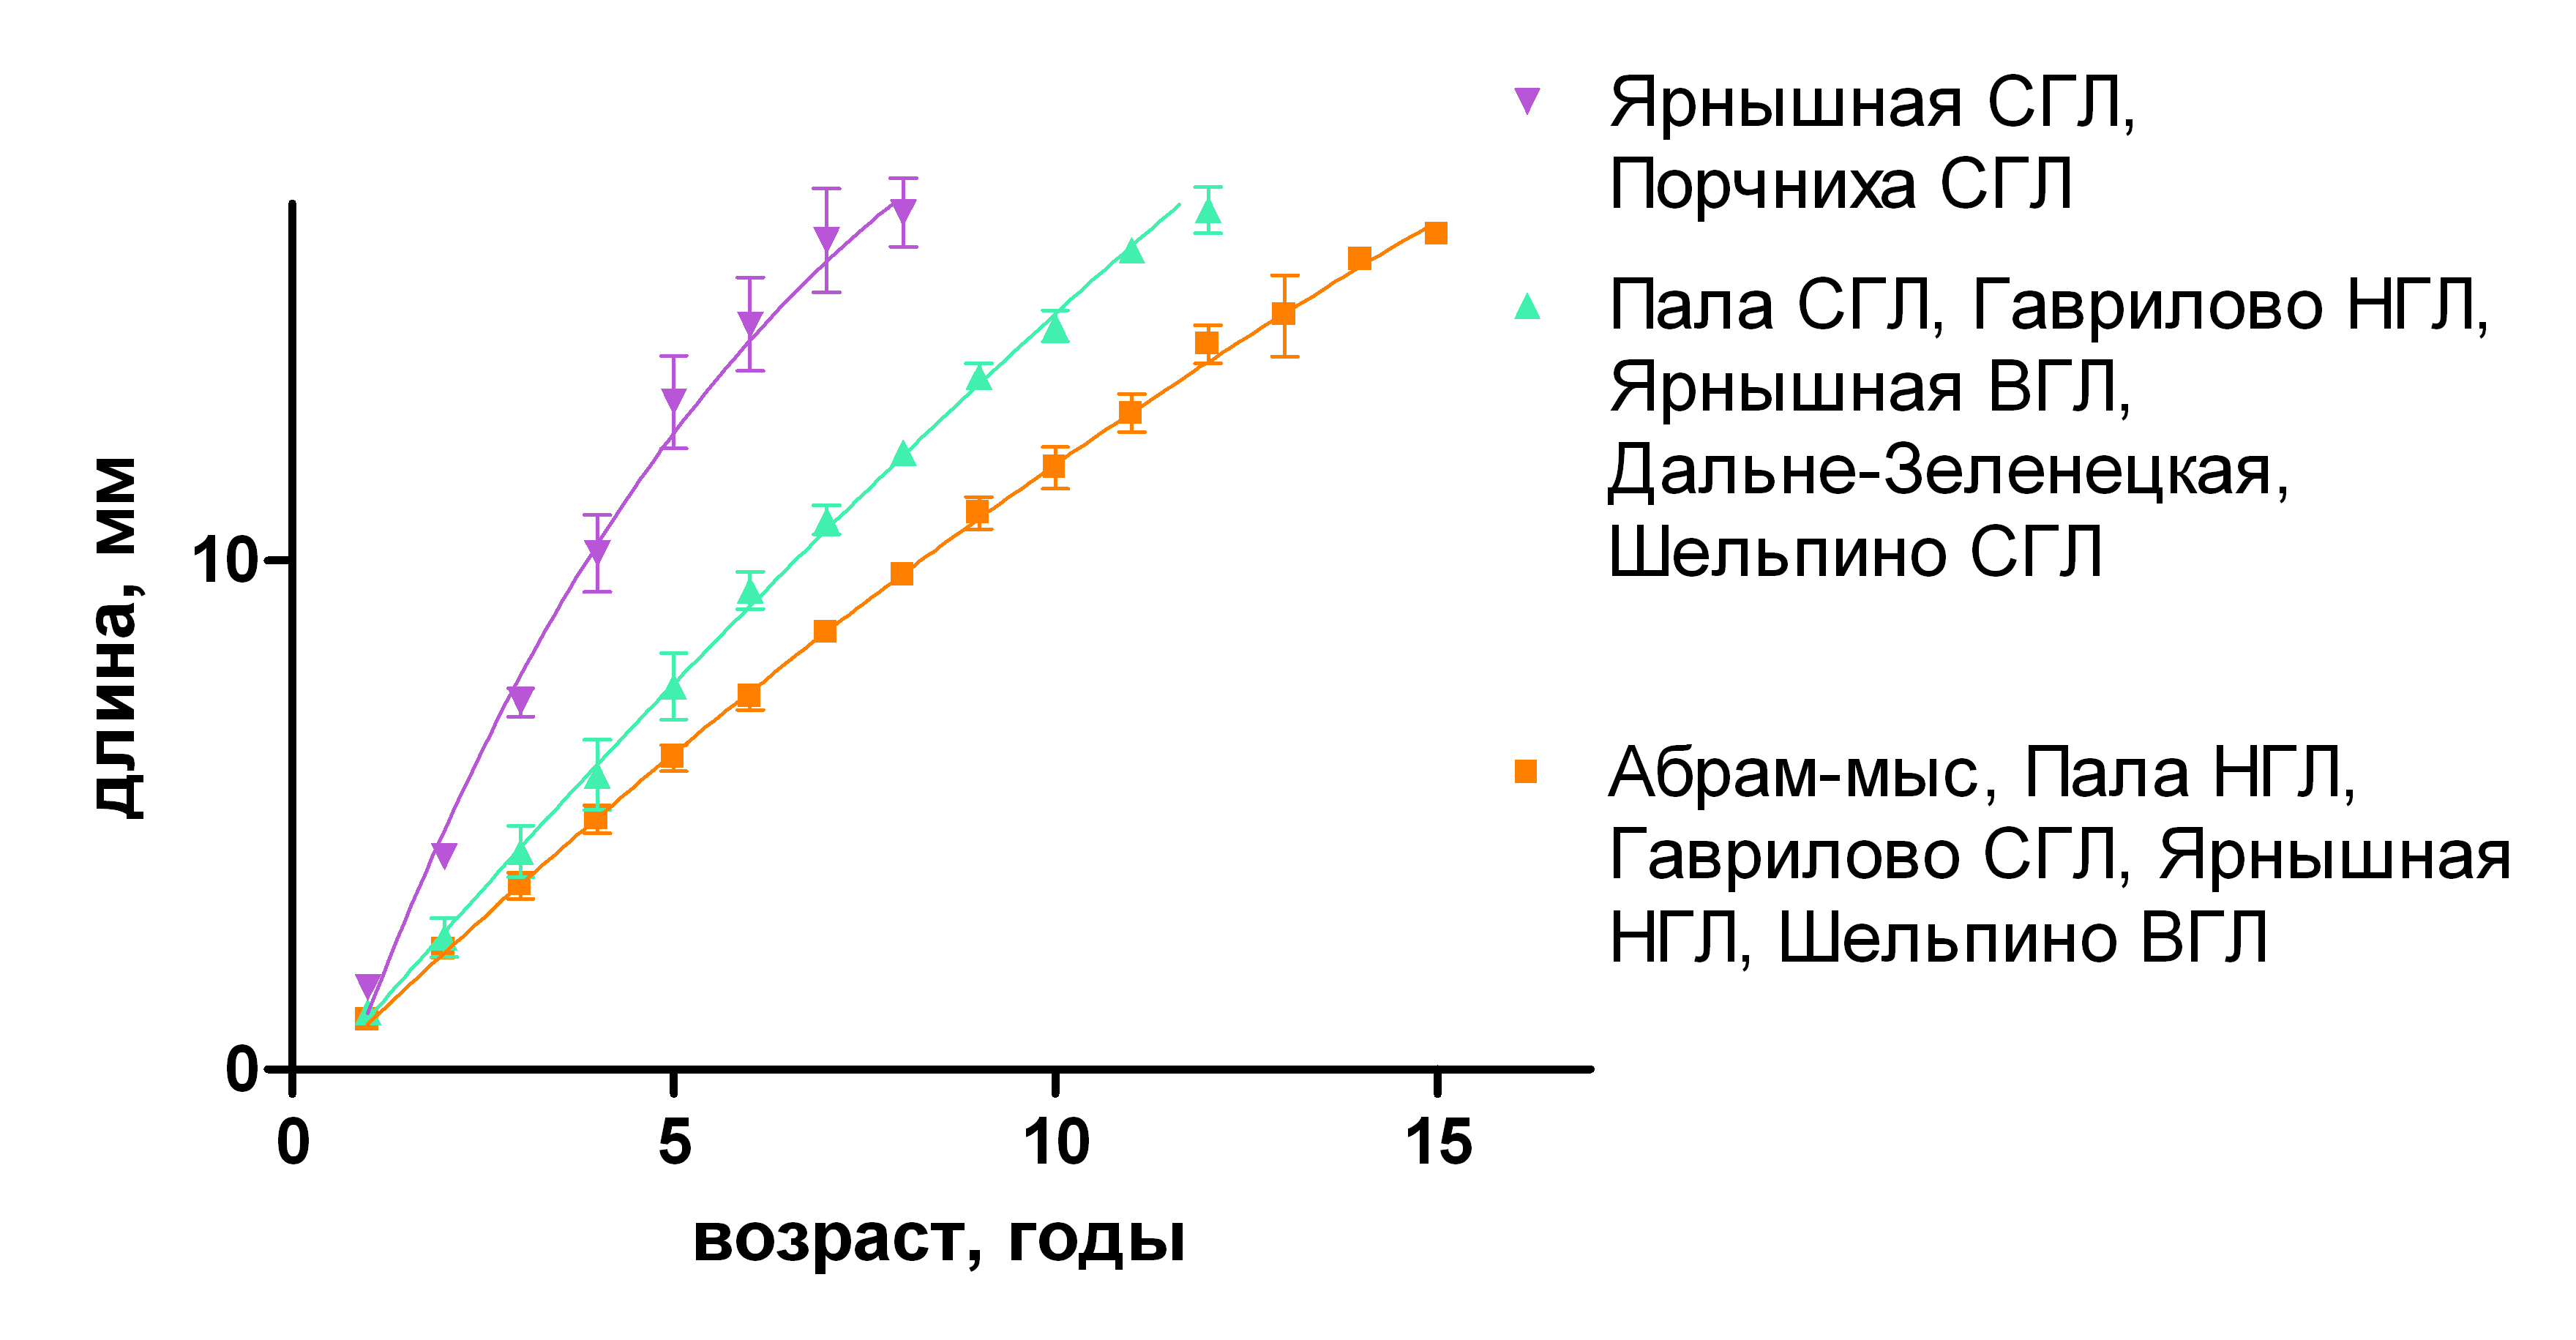
\includegraphics[width=\textwidth]{../Barenc_Sea/growth_from_MSc/rost_clusters_all.jpg}
    \caption{Модели роста, передающие  принципиальные свойства вариации характера линейного роста маком в изученных местообитаниях}
    \label{ris:Barents_clusters_gorizonts_all}
    \end{figure}
Первая группа — особи с наименьшей скоростью роста достигали длины $16,4$ мм за $14$ лет, обитавшие на относительно более низком уровне осушки. 
Макомы с промежуточной   скоростью   роста   вырастали   за   $13$   лет   $до   19,3$   мм.   
Особи   с   максимальной скоростью роста за $9$ лет достигали длины $18$ мм.

Таким   образом,   не   удалось   выделить   ни   географической,   ни   мареографической приуроченности особей с одинаковой скоростью роста. 
Возможно, это связано с тем, что во взвешенных оценках возрастных рядов могут сильнее проявиться черты нехарактерных, но сильно   представленных   в   поселении   сегодня   генераций,   и,   следовательно,   в   каждом возрастном   ряду   получается   разная   представленность   межгодовой   составляющей   условий 
роста маком. 

Для   того,   чтобы   снять   эти   влияния,   следующий   анализ   проводили   с   купированием исходных  данных  до  объединения   нескольких  описаний возрастных рядов  только  старших (>8+) генераций (рис.~\ref{ris:Barents_growth_gorizonts_8year}).
    \begin{figure}[p]
        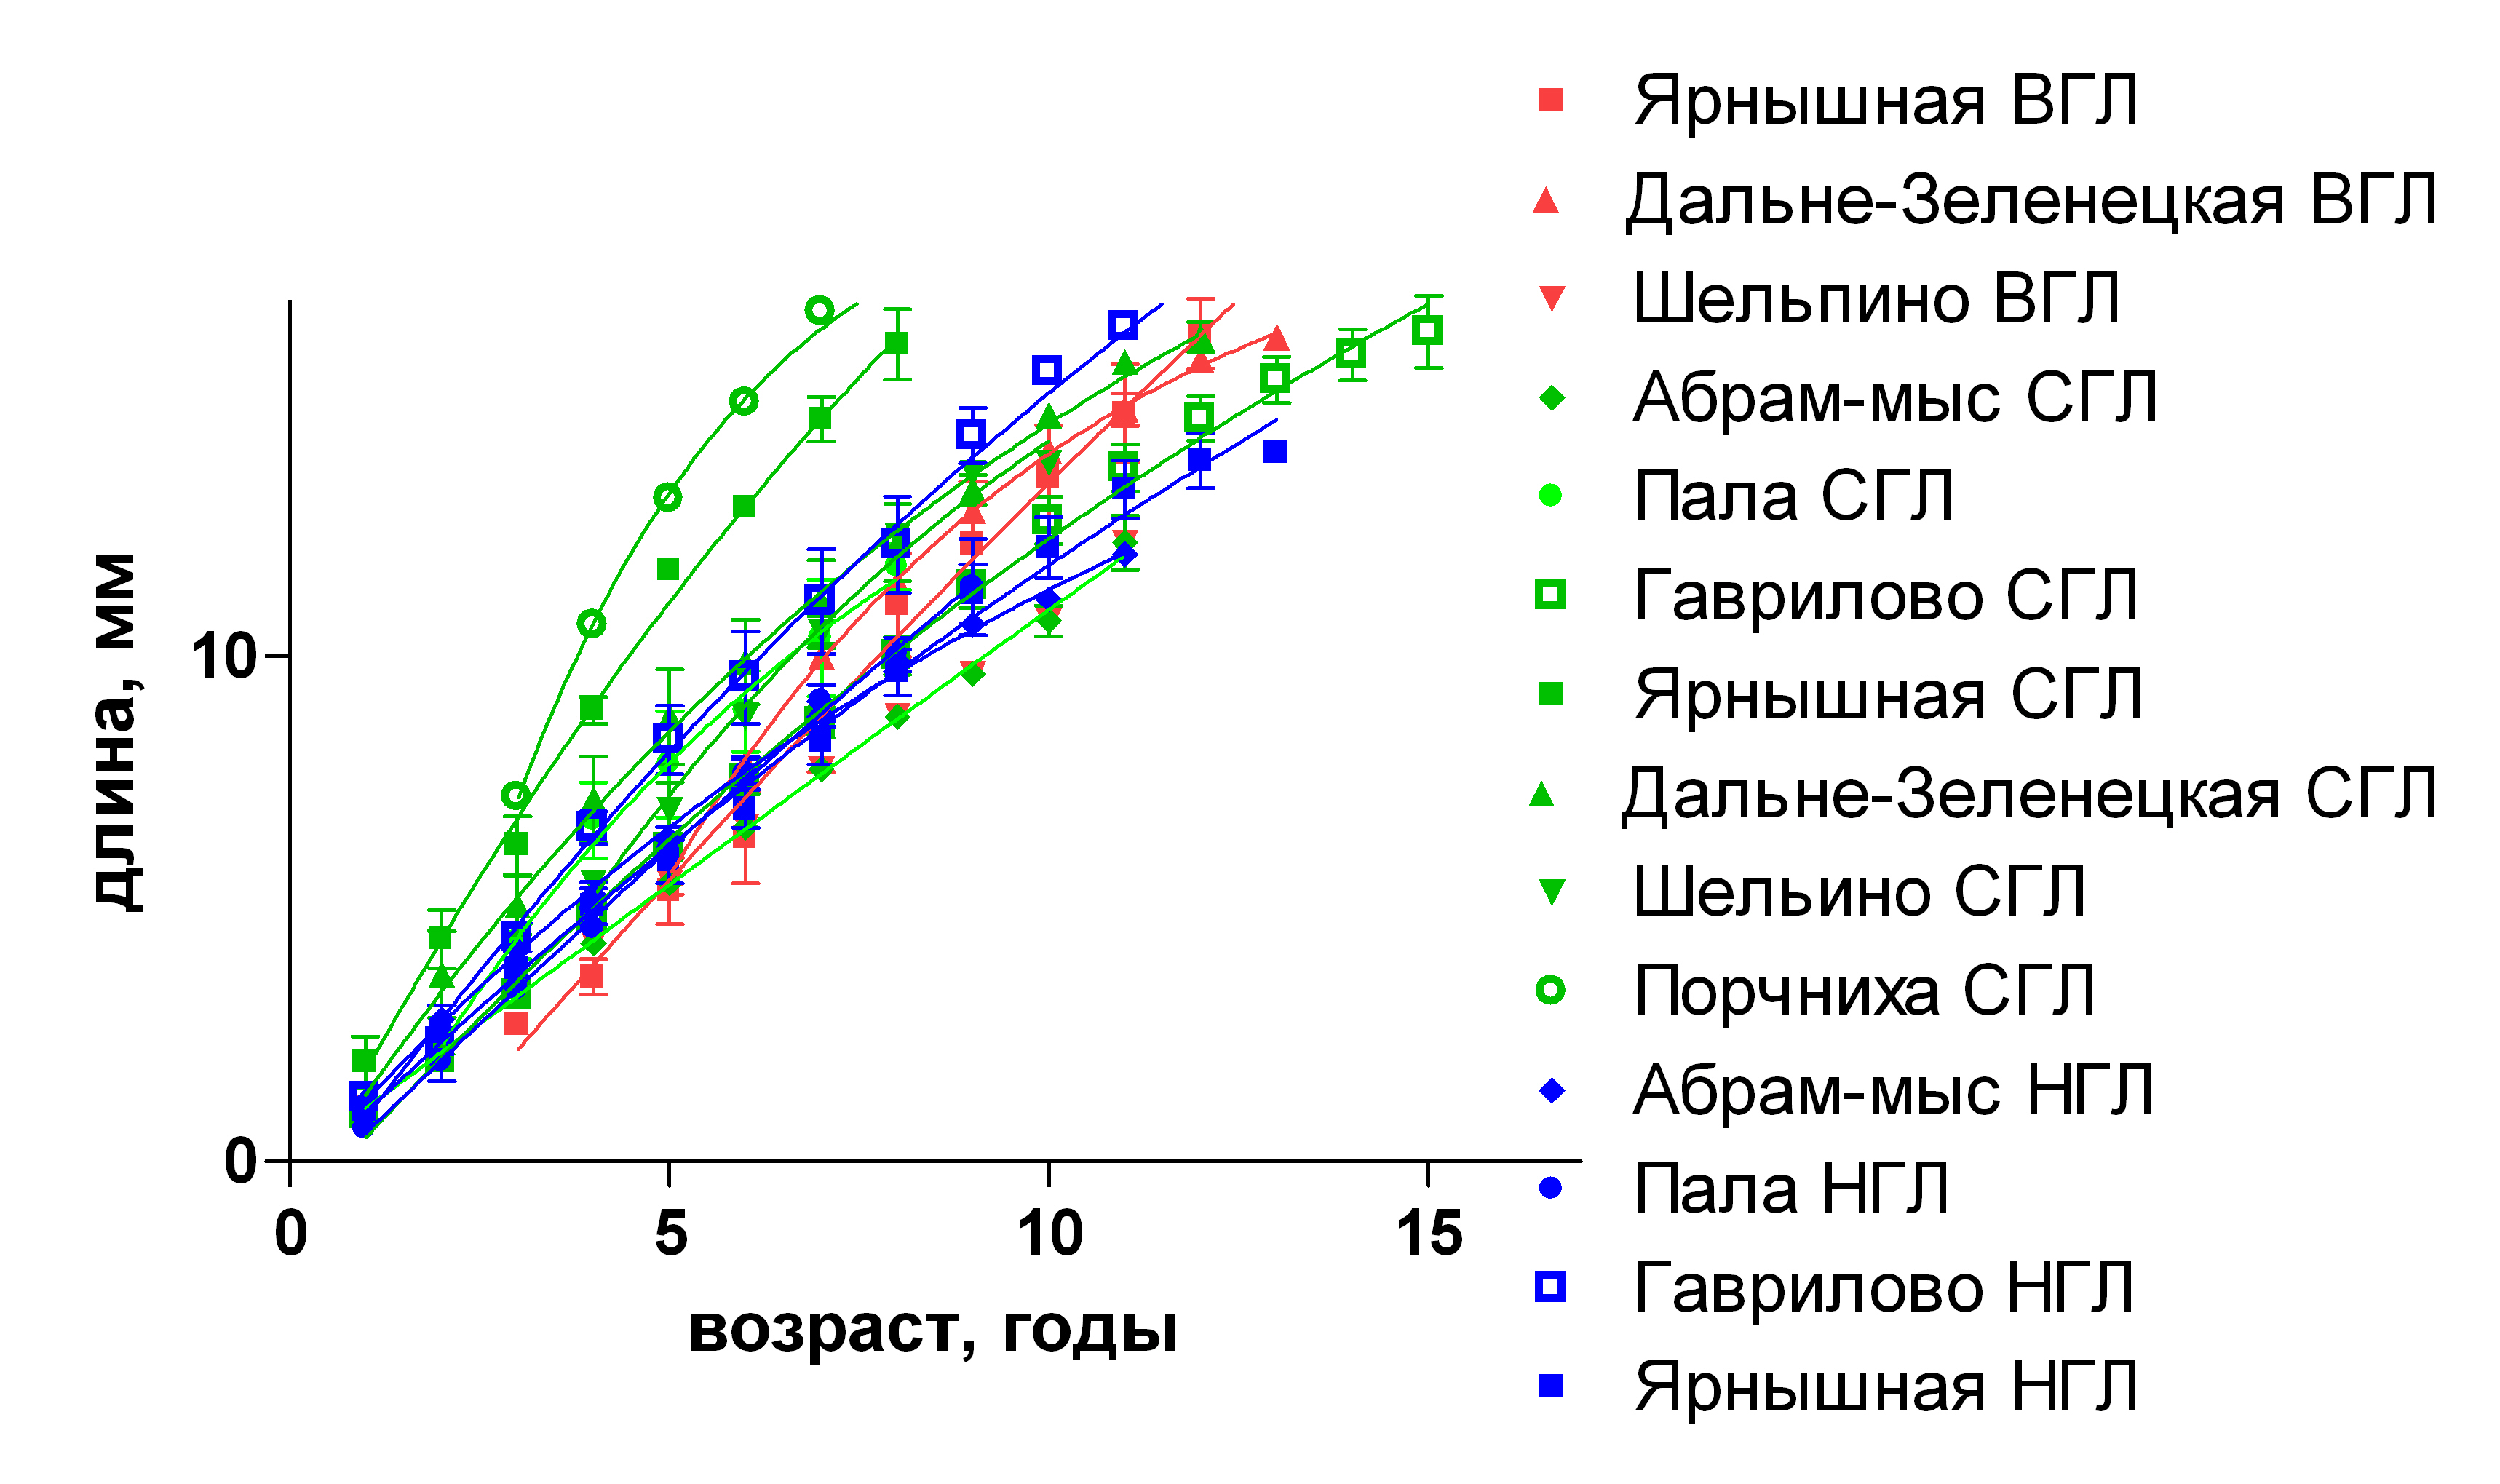
\includegraphics[width=\textwidth]{../Barenc_Sea/growth_from_MSc/Rost_8+_gorizonts.jpg}
        \caption{Разнообразие моделей линейного роста, описывающих усредненные возрастные ряды генераций маком старше 8 лет} 
    \label{ris:Barents_growth_gorizonts_8year}
    \end{figure}
Полученная   картина   аналогична   полученной   по   интегральным   описаниям:   быстрее всего росли макомы в среднем горизонте литорали губы Порчниха и в среднем горизонте литорали губы Ярнышная, в то время как остальные кривые не распадаются на очевидные группы, и некоторые пересекают друг друга. 
Однако при сравнении полученных кривых роста с учетом разброса эмпирических данных относительно регрессионной модели было выделено 4 кластера (рис.~\ref{ris:dendrogramma_linear_clusters_8year}).
    \begin{figure}[p]
        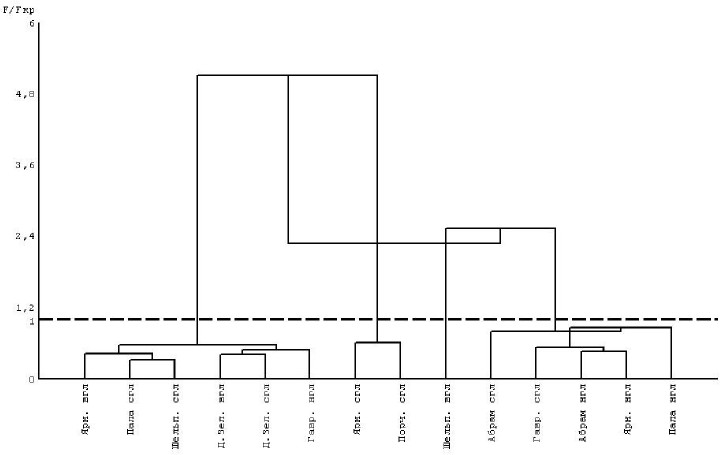
\includegraphics[width=\textwidth]{../Barenc_Sea/growth_from_MSc/dendrogramma_sravnenie_rosta_linear_8year_gorizonts.jpg}
        \caption{Классификация поселений маком по моделям линейного роста, описывающих усредненные возрастные ряды генераций маком старше 8 лет}
    \label{ris:dendrogramma_linear_clusters_8year}
    \end{figure}

В первый кластер (уровень различий внутри кластера менее $0,86$) вошли следующие описания:  Абрам-мыс, Пала-губа НГЛ, губа  Гаврилово  СГЛ, губа Ярнышная НГЛ. 
Второй кластер (уровень различий внутри кластера менее $0,57$) составили участки Пала-губа СГЛ, губа Гаврилово НГЛ, губа Дальне-Зеленецкая, губа Ярнышная ВГЛ, Шельпино СГЛ. 
В третий кластер (уровень различий внутри кластера менее $0,61$) вошли участки губа Ярнышная СГЛ и губа Порчниха СГЛ. 
В отдельный кластер попал участок губа Шельпино ВГЛ (минимальное различие $2,53$ --- с кластером $1$). 
Таким   образом,   единственное   качественное   изменение   относительно   результатов, полученных при сравнении усредненных кривых роста --- это выделение верхнего горизонта литорали губы Шельпино в отдельный кластер. 
Однако, коэффициенты различия значительно изменились. 
В два раза увеличилось различие между описаниями внутри кластера $3$, различие внутри кластера $2$ уменьшились. 
Максимальное различие было отмечено между кластерами два и три ($5,1$).

По итогам классификации было выделено четыре группы маком, отличающиеся по характеру роста (рис. \ref{ris:Barents_clusters_gorizonts_8year}). 
    \begin{figure}[p]
        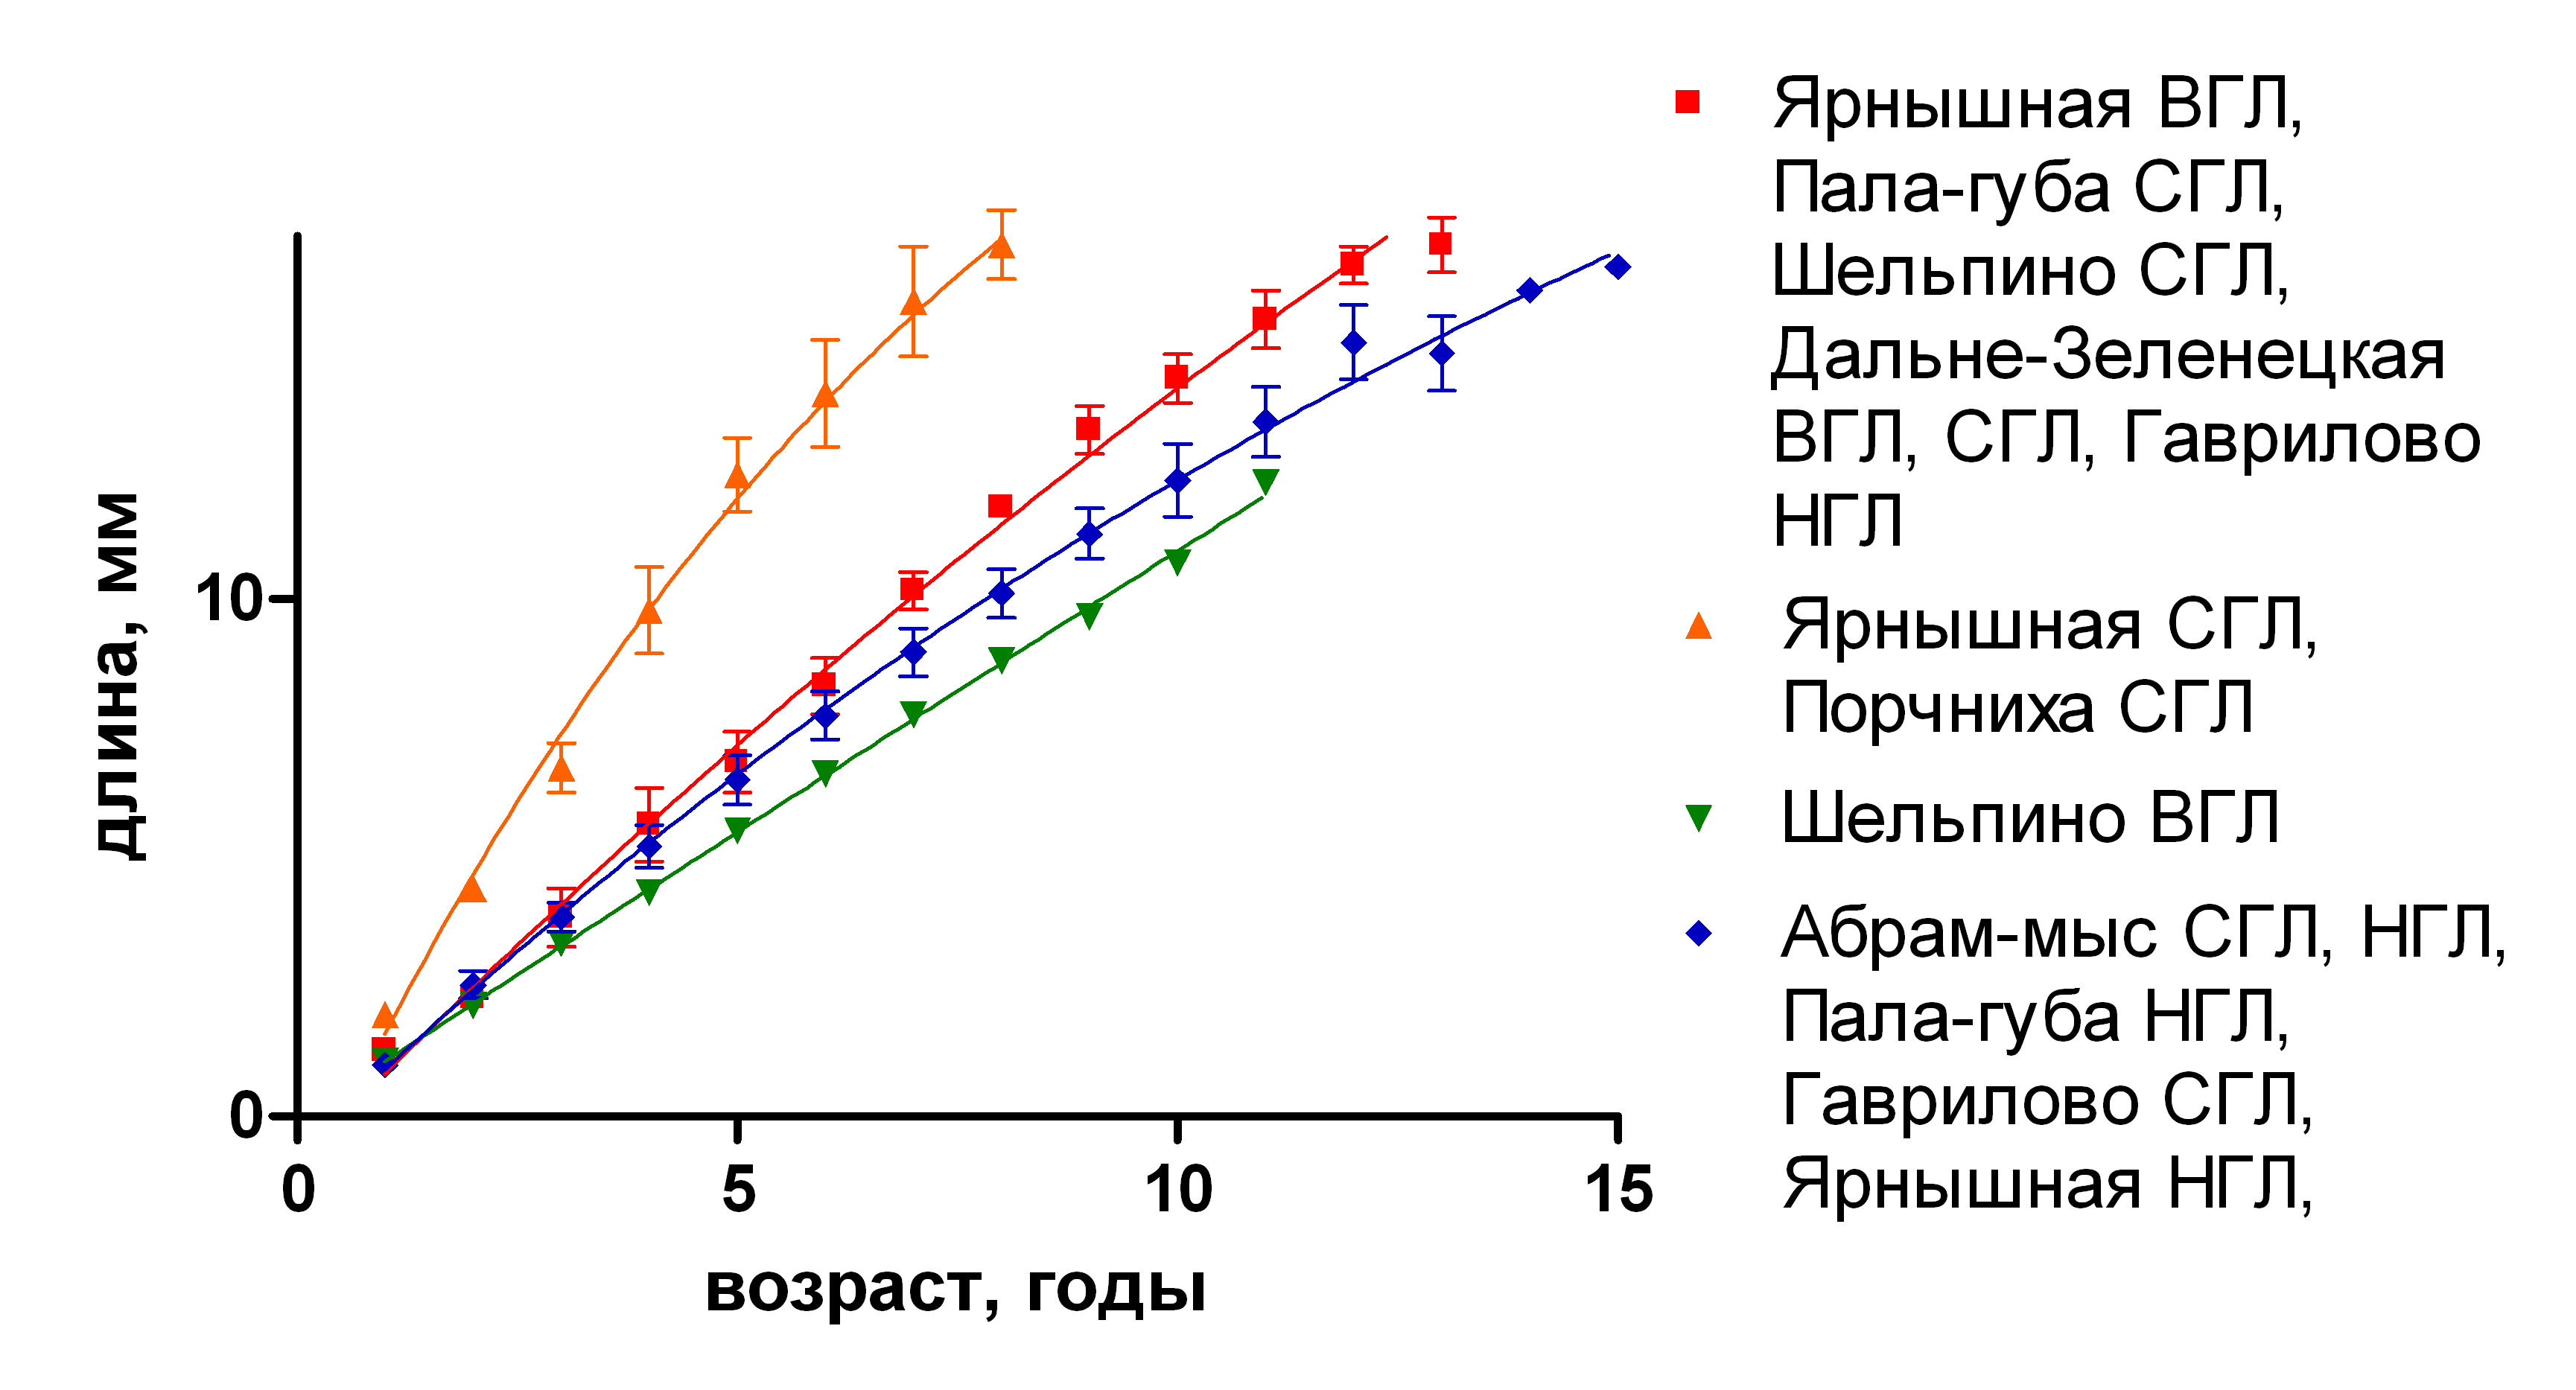
\includegraphics[width=\textwidth]{../Barenc_Sea/growth_from_MSc/Rost_8+_clusters.jpg}
        \caption{Модели роста, передающие  принципиальные свойства вариации характера  линейного роста маком старше 8 лет в изученных местообитаниях}
    \label{ris:Barents_clusters_gorizonts_8year}
    \end{figure}
Особи с минимальной скоростью роста ($14$~мм за $12$~лет) обитали в верхнем горизонте литорали губы Шельпино.
Среди групп с промежуточной скоростью роста более   низкой   скоростью   роста   ($16,4$~мм   за   $14$~лет)   обладали   моллюски,   обитавшие   на относительно более низком уровне осушки. 
Особи с максимальной скоростью роста за $9$ лет достигали длины $18$ мм.

Использование   интегральных   моделей   роста   маком   вполне   отвечает   задаче сравнительного анализа их поселений. 
Однако скорость роста моллюсков зависит не только от внешних,   общих   для   всего   поселения,   факторов,   но   и   от   локальных   микроусловий.      
Материалы   настоящей   работы   не   позволяют   нам   провести   анализ   вариации индивидуальных   особенностей   роста   маком   как   отклика   на   условия   их   роста.   
Для   этого нужны специальные экспериментальные исследования. 
Однако можно попытаться выделить групповые   эффекты.   
Речь   идет   о   снижении   уровня   рассматриваемой   биосистемы   до возрастной группы. 

В таблицах приложения~\ref{app:growth_matrix} приведены усредненные для каждой возрастной группы результаты измерений  расстояния  от верхушки раковины до каждой метки  зимней остановки роста.
Используем их для анализа характера вариации средних величин годового прироста. 
Величины годового прироста варьировали от $0,05$ до $3,58$ мм (табл.~\ref{tab:godovoy_prirost_min_max}).
\begin{table}[p]
    \caption{Размах варьирования годового прироста {\it Macoma balthica} в зависимости от участка, горизонта     литорали и начального размера особи}
    \label{tab:godovoy_prirost_min_max}
    \begin{tabularx}{\textwidth}{|lX|XX|XX|XX|XX|}
        \hline
        Участок        &         & \multicolumn{8}{c|}{начальный размер}                                             \\ \cline{3-10}
                              &                 & \multicolumn{2}{c|}{$< 3$ мм} & \multicolumn{2}{c|}{$3-6$ мм} & \multicolumn{2}{c|}{$6-9$ мм} &\multicolumn{2}{c|}{$> 9$ мм}\\ \hline
     \multicolumn{2}{|r|}{годовой прирост}&  мин              & макс   & мин    & макс              & мин  & макс & мин  & макс \\ \hline
        Абрам-мыс      & сгл             & 0,69             & 1,68   & 0,69   & 1,31              & 0,73 & 1,57 & 1,00 & 1,23 \\
                       &  нгл            & 0,90            & 1,77             & 0,88   & 1,48   & 0,80              & 1,73 & 0,67 & 1,50 \\ \hline
        Пала-губа      & сгл             & 0,77             & 2,15   & 1,20   & 2,90              & 1,05 & 1,68 & 1,40 & 1,40 \\
                       & нгл            & 1,01            & 1,43             & 1,01   & 1,86   & 0,83              & 1,73 & 0,85 & 0,85 \\ \hline
        губа Гаврилово & сгл             & 0,70             & 2,10   & 0,93   & 2,40              & 0,80 & 2,10 & 0,70 & 1,75 \\
                       &  нгл            & 0,60            & 2,30             & 1,00   & 2,20   & 0,80              & 2,10 & 0,60 & 1,90 \\ \hline
        губа Ярнышная  & сгл             & 1,08             & 3,30   & 1,80   & 3,58              & 2,60 & 2,75 & 1,22 & 2,52 \\
                       &  нгл            & 0,80            & 1,60             & 0,80   & 1,50   & 0,95              & 1,56 & 0,05 & 1,72 \\   \hline
    \end{tabularx}
\end{table}

В качестве переменных воздействия в контексте данной работы логично обратиться к  таким   причинам   вариации   скорости   маком   как   география   положения   местообитаний, мареография положения станций наблюдений. 
Кроме того, нельзя не учесть очевидную связь величины годового прироста маком с их возрастом. 

В   проведенном   выше   сравнительном   анализе   интегральных   кривых   роста   мы выравнивали эмпирические возрастные ряды с помощью линейной модификации уравнения роста Берталанфи. 
При этом очевидным образом снижается объективность представлений о межгодовых различиях годовых приростов особей в возрастных группах. 
Попробуем отойти от возраста как от условия, организующего скорость роста маком, и в качестве одного из предикторов   величины   годового   прироста   возьмём   начальный   (к   данному   годовому интервалу) средний размер особей возрастной группы.  
Такой анализ логично провести с помощью дисперсионного анализа. 

%из статьи
На первом этапе анализа (факторы <<горизонт литорали>>, <<начальный средний размер особей в возрастной группе>>) установлено (табл.~\ref{tab:prirost_ANOVA_tidal}), что каждая из назначенных причин вариации достоверно определяет величину годового прироста. 
\begin{table}[p]
    \caption{Структура вариансы средних величин годового прироста {\it M. balthica} в возрастных группах в градиентах величины начального среднего размера особей в возрастной группе и мареографического уровня положения станций наблюдения}
    \label{tab:prirost_ANOVA_tidal}
    \begin{center}
    \begin{tabular}{|l|rrrrr|}
    \hline
    Источник вариации & $SS$   & $\nu$   & $M_S$   & $F$     & $\alpha$     \\ \hline
    A                 & 4,74   & 3   & 1,58 & 4,2   & 0,006 \\
    B                 & 11,98  & 2   & 5,99 & 15,92 & 0     \\
    AB                & 2,75   & 6   & 0,46 & 1,22  & 0,295 \\
    W                 & 193,82 & 515 & 0,38 &       &       \\ \hline
\end{tabular}
\end{center}

    \footnotesize{Источники вариации: А --- величины начального среднего размера особей в возрастной группе (4 градации размерных классов),\\ 
    В --- мареографический уровень положения станций наблюдения (три градации)\\
    W --- внутригрупповая вариация.\\
    $SS$ --- общий квадрат, $\nu$ --- степень свободы, $M_S$ --- средний квадрат (варианса), $F$ --- значение статистики Фишера, $\alpha$ --- уровень значимости критерия.}
\end{table}
Весьма примечательно, что при этом наибольшая доля вариации величин годового прироста определяется не начальным размером маком ($SS = 4,74$), а мареографическим уровнем положения станции ($SS = 11,98$).
При анализе структуры вариансы исходного комплекса в градиентах начального среднего размера особей в возрастной группе и географии местообитаний выяснилось, что достоверное влияние на величину среднего годового прироста маком оказывают также оба фактора (табл.~\ref{tab:prirost_ANOVA_geography}).
\begin{table}[p]
    \caption{Структура вариансы средних величин годового прироста {\it M. balthica} в возрастных группах в градиентах величины начального среднего размера особей в возрастной группе и географического положения участка наблюдений}
    \label{tab:prirost_ANOVA_geography}
    \begin{center}
    \begin{tabular}{|l|rrrrr|}
        \hline
    Источник вариации & $SS$   & $\nu$   & $M_S$   & $F$     & $\alpha$     \\ \hline
        A                 & 8,23   & 2   & 4,12 & 13,14 & 0,000003 \\
        C                 & 14,44  & 5   & 2,89 & 9,22  & 0        \\
        AC                & 14,16  & 17  & 0,83 & 2,66  & 0,000351 \\
        W                 & 156,62 & 500 & 0,31 &       &         \\ \hline
    \end{tabular}
\end{center}

    \footnotesize{Источники вариации: А --- величины начального среднего размера особей в возрастной группе (4 градации размерных классов),\\ 
        C --- географическое положение участка наблюдений (6 градаций)\\
    W --- внутригрупповая вариация.\\
    $SS$ --- общий квадрат, $\nu$ --- степень свободы, $M_S$ --- средний квадрат (варианса), $F$ --- значение статистики Фишера, $\alpha$ --- уровень значимости критерия.}
\end{table}
Причем и в этом случае наибольшая доля вариации обусловлена не начальным размером раковины, а фактором <<участок>> ($SS = 14,44$).
Общим для проведенных вариантов двухфакторного дисперсионного анализа оказалось, что в обоих случаях внутригрупповая вариация на порядок превышает факторную составляющую. 
Это говорит о том, что основной причиной вариации величины годового прироста маком в изученных акваториях является крайняя степень разнокачественности особей в местообитаниях. 
%Такая разнокачественность очевидна уже по величине размаха вариации длины раковины маком в возрастных группах (см. табл. 1).
В качестве рабочей гипотезы можно предположить, что в краевой части ареала резкой дифференциации особей {\it M. balthica} по скорости роста могут способствовать любые проявления микрорельефной гетеротопности локальных местообитаний.
Полученные положительные итоги дисперсионного анализа интересно визуализировать для выявления характера мареографического и географического трендов в изменении величины годового прироста маком. 
Для этого представим итоги двухфакторных дисперсионных анализов в виде соответствующих поверхностей отклика.
Весьма показательно, что величины годового прироста маком по мере увеличения начального среднего размера особей в возрастных группах меняются куполообразно (рис.~\ref{ris:prirost_otklik}). 
	\begin{figure}[p]
		\begin{minipage}[b]{.5\linewidth}
		%Фигурка в первом ряду слева размер отведенный под весь этот объект -- 0.46 от ширины строки
		%Параметр [b] означает, что выравнивание этих министраниц будет по нижнему краю
			\begin{center}
				{\small А}
				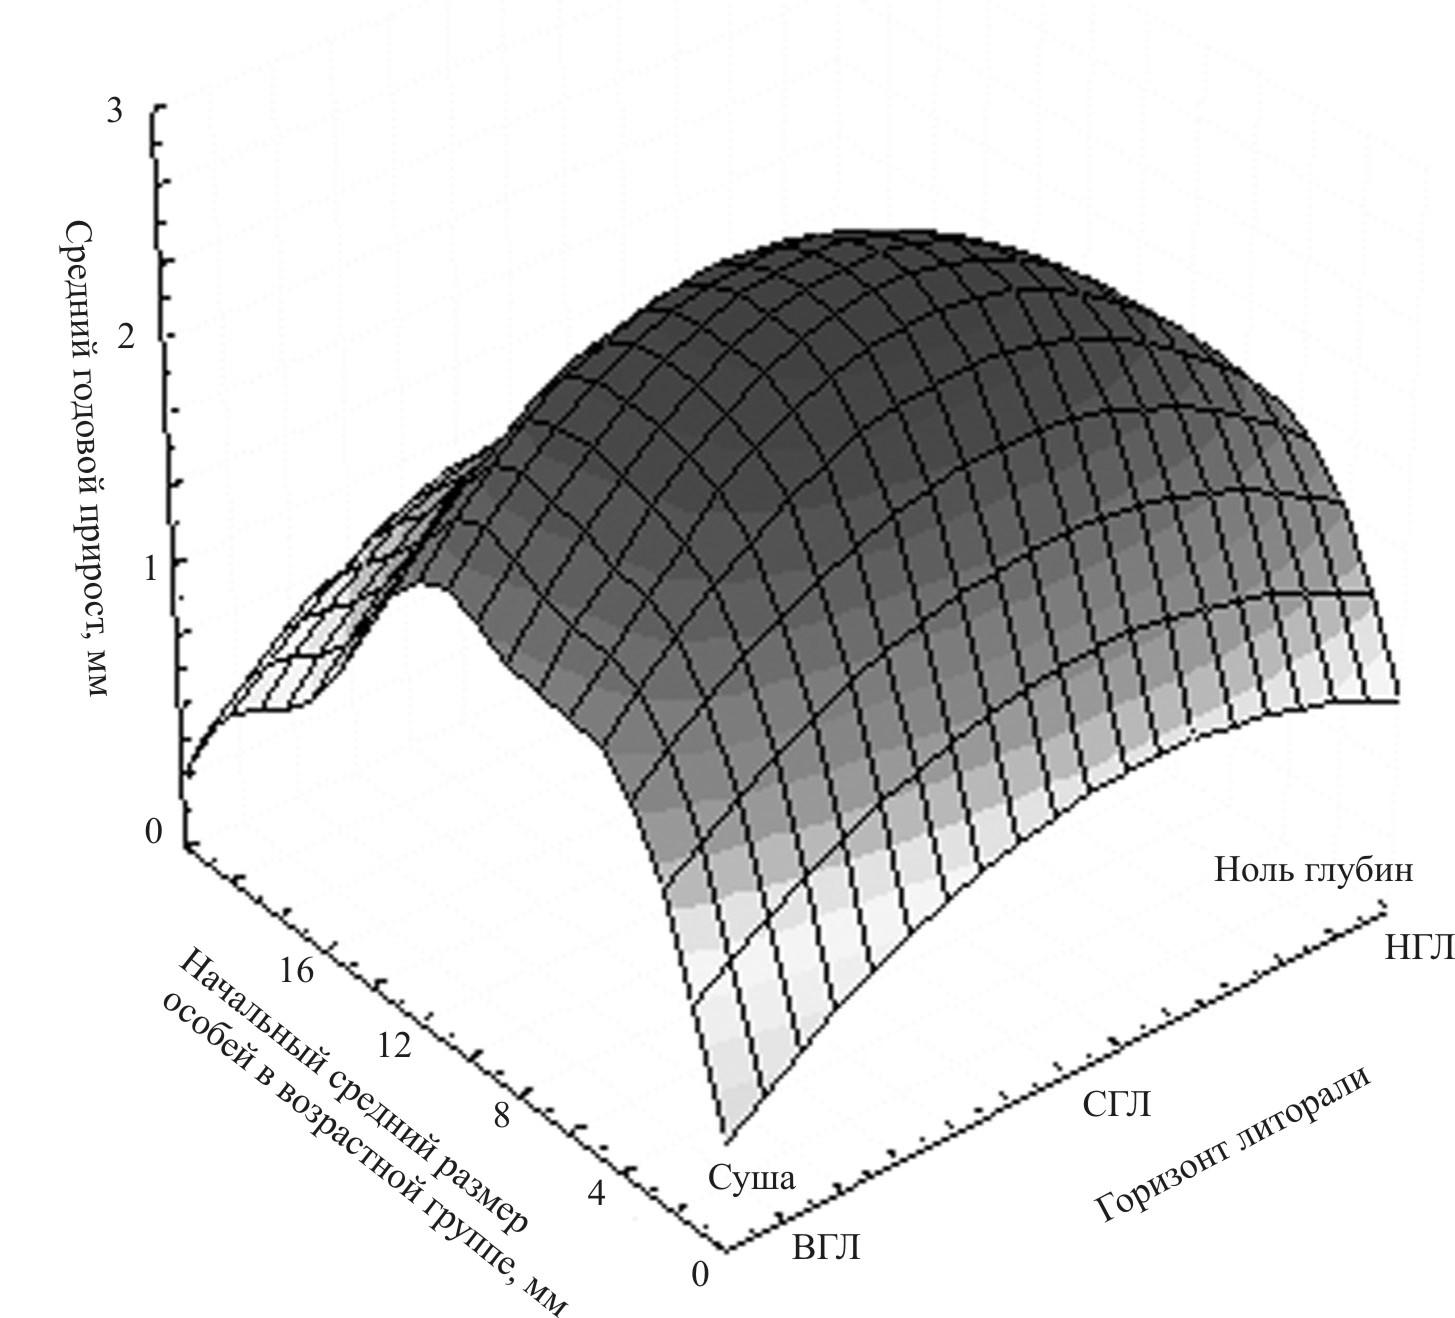
\includegraphics[width=70mm]{../Barenc_Sea/growth_from_MSc/prirost_otklik_mareography.jpg}
			\end{center}
		\end{minipage}
	\hfil %Это пружинка отодвигающая рисунки друг от друга
		\begin{minipage}[b]{.5\linewidth}
			\begin{center}
				{\small B}
				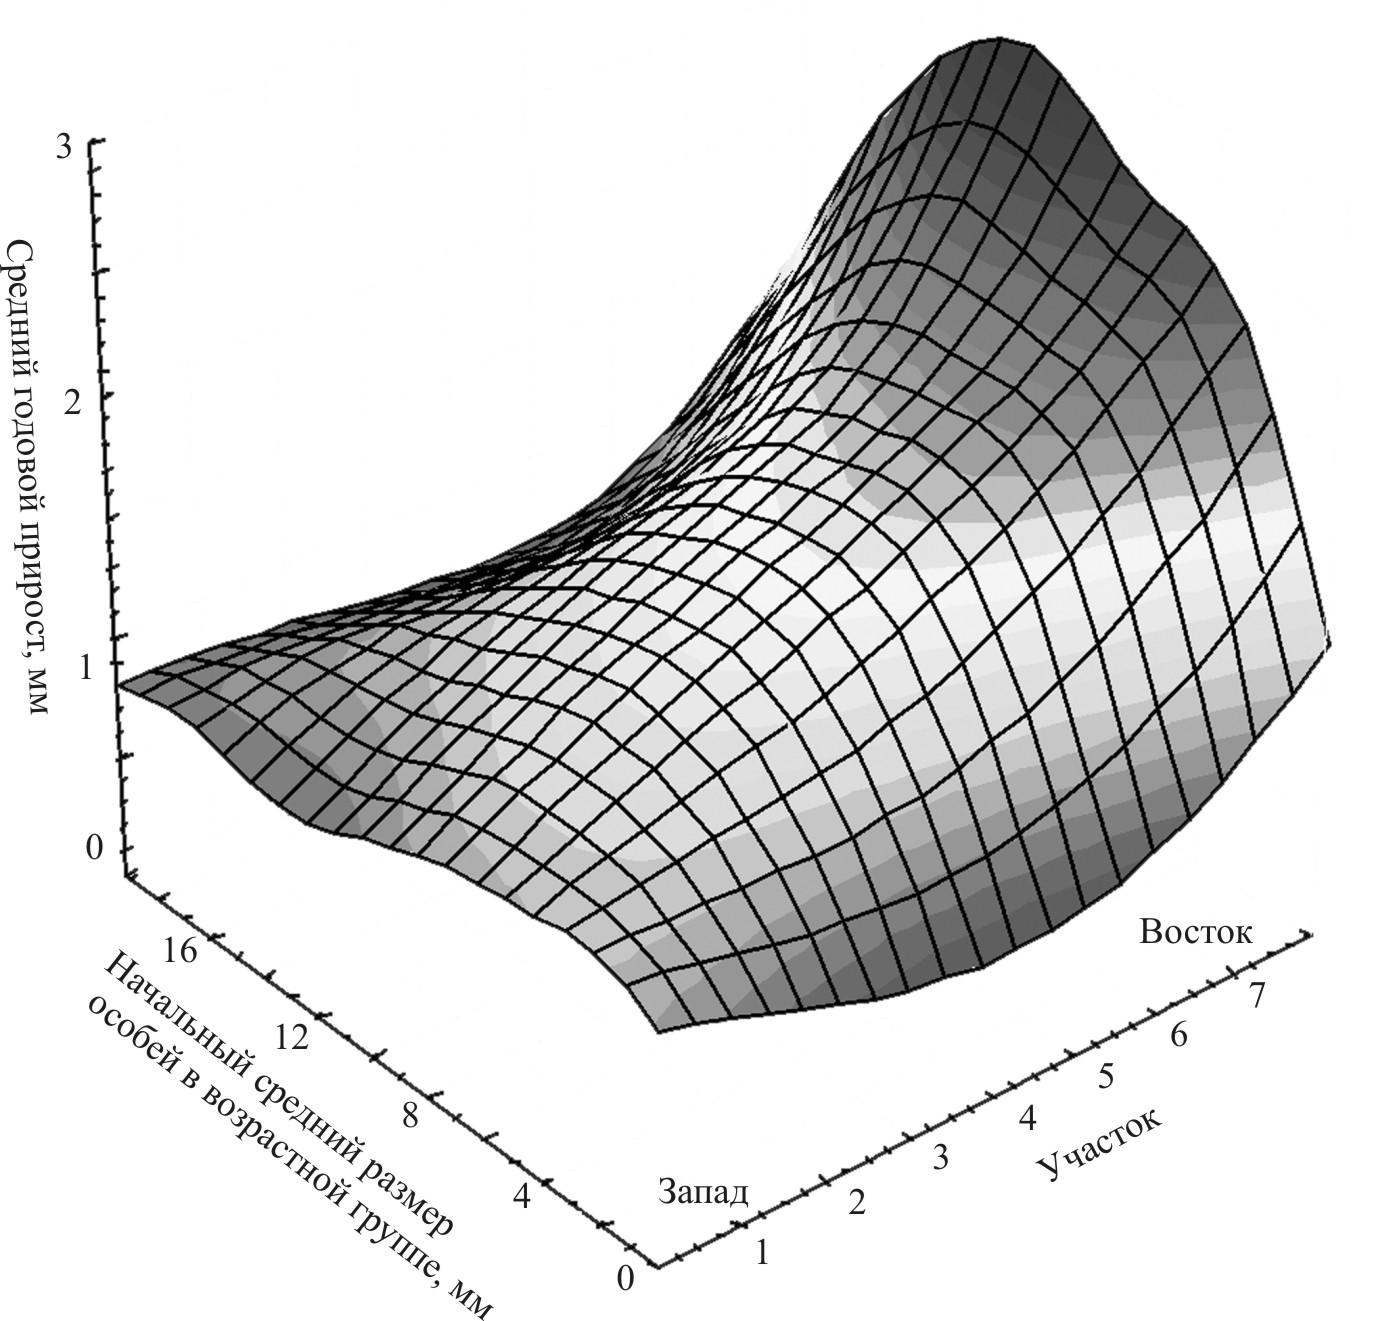
\includegraphics[width=70mm]{../Barenc_Sea/growth_from_MSc/prirost_otklik_geography.jpg}
			\end{center}
		\end{minipage}
	\caption{Характер изменений средней величины годового прироста особей {\it Macoma balthica} возрастной группы в зависимости от начальной средней длины их раковин, мареографического уровня обитания (A) и условного смещения участка по побережью Мурмана на восток (B)}
\footnotesize{Примечания: Участки: 1 --- Абрам-мыс, 2 --- Пала-губа, 3 --- Гаврилово, 4 --- Ярнышная, 5 --- Дальне-Зеленецкая, 6 --- Шельпино, 7 --- Порчниха\\
ВГЛ --- верхний горизонт литорали, СГЛ --- средний горизонт литорали, НГЛ --- нижний горизонт литорали}
	\label{ris:prirost_otklik}
	\end{figure}
Во всех исследованных поселениях максимальный прирост наблюдается у особей размерного класса $6 - 9$~мм. 
Таким образом, в изученных поселениях максимальную скорость роста следует ожидать у маком среднего возраста (размера). 
Совершенно неожиданным для нас было явление максимальной скорости роста маком не в нижнем, а в среднем горизонте осушной зоны (см. рис.~\ref{ris:prirost_otklik}, А). 
%По-видимому, в условиях Мурмана фактор осушки начинает оказывать заметное влияние на скорость роста маком только в верхнем горизонте литорали. 
%Причины снижения скорости роста маком в условиях нижнего горизонта литорали на данном этапе исследований нам не ясны.

\bigskip
Таким образом, на литорали Баренцева моря особи \textit{M.~balthica} гетерогенны по скорости роста.
При сравнении кривых роста не было отмечено сходства роста у особей из одного поселения или с одного уровня осушки. 
Однако анализ среднего годового прироста в различных размерных группах показал, что в более восточных поселениях данный показатель выше, чем в более западных.
Также было показано, что в среднем горизонте литорали средний годовой прирост оказывается выше, чем в верхнем и нижнем.
Данные закономерности были выражены в разной степени у особей, отличающихся по длине раковины.
Во всех случаях наибольший средний годовой прирост наблюдали у особей с длиной раковины $6 - 9$~мм.

\afterpage{\clearpage}
